% Options for packages loaded elsewhere
\PassOptionsToPackage{unicode}{hyperref}
\PassOptionsToPackage{hyphens}{url}
%
\documentclass[
  ignorenonframetext,
]{beamer}
\title{Tema 1 - Probabilidad}
\author{}
\date{\vspace{-2.5em}}

\usepackage{pgfpages}
\setbeamertemplate{caption}[numbered]
\setbeamertemplate{caption label separator}{: }
\setbeamercolor{caption name}{fg=normal text.fg}
\beamertemplatenavigationsymbolsempty
% Prevent slide breaks in the middle of a paragraph
\widowpenalties 1 10000
\raggedbottom
\setbeamertemplate{part page}{
  \centering
  \begin{beamercolorbox}[sep=16pt,center]{part title}
    \usebeamerfont{part title}\insertpart\par
  \end{beamercolorbox}
}
\setbeamertemplate{section page}{
  \centering
  \begin{beamercolorbox}[sep=12pt,center]{part title}
    \usebeamerfont{section title}\insertsection\par
  \end{beamercolorbox}
}
\setbeamertemplate{subsection page}{
  \centering
  \begin{beamercolorbox}[sep=8pt,center]{part title}
    \usebeamerfont{subsection title}\insertsubsection\par
  \end{beamercolorbox}
}
\AtBeginPart{
  \frame{\partpage}
}
\AtBeginSection{
  \ifbibliography
  \else
    \frame{\sectionpage}
  \fi
}
\AtBeginSubsection{
  \frame{\subsectionpage}
}
\usepackage{amsmath,amssymb}
\usepackage{lmodern}
\usepackage{iftex}
\ifPDFTeX
  \usepackage[T1]{fontenc}
  \usepackage[utf8]{inputenc}
  \usepackage{textcomp} % provide euro and other symbols
\else % if luatex or xetex
  \usepackage{unicode-math}
  \defaultfontfeatures{Scale=MatchLowercase}
  \defaultfontfeatures[\rmfamily]{Ligatures=TeX,Scale=1}
\fi
% Use upquote if available, for straight quotes in verbatim environments
\IfFileExists{upquote.sty}{\usepackage{upquote}}{}
\IfFileExists{microtype.sty}{% use microtype if available
  \usepackage[]{microtype}
  \UseMicrotypeSet[protrusion]{basicmath} % disable protrusion for tt fonts
}{}
\makeatletter
\@ifundefined{KOMAClassName}{% if non-KOMA class
  \IfFileExists{parskip.sty}{%
    \usepackage{parskip}
  }{% else
    \setlength{\parindent}{0pt}
    \setlength{\parskip}{6pt plus 2pt minus 1pt}}
}{% if KOMA class
  \KOMAoptions{parskip=half}}
\makeatother
\usepackage{xcolor}
\IfFileExists{xurl.sty}{\usepackage{xurl}}{} % add URL line breaks if available
\IfFileExists{bookmark.sty}{\usepackage{bookmark}}{\usepackage{hyperref}}
\hypersetup{
  pdftitle={Tema 1 - Probabilidad},
  hidelinks,
  pdfcreator={LaTeX via pandoc}}
\urlstyle{same} % disable monospaced font for URLs
\newif\ifbibliography
\usepackage{longtable,booktabs,array}
\usepackage{calc} % for calculating minipage widths
\usepackage{caption}
% Make caption package work with longtable
\makeatletter
\def\fnum@table{\tablename~\thetable}
\makeatother
\usepackage{graphicx}
\makeatletter
\def\maxwidth{\ifdim\Gin@nat@width>\linewidth\linewidth\else\Gin@nat@width\fi}
\def\maxheight{\ifdim\Gin@nat@height>\textheight\textheight\else\Gin@nat@height\fi}
\makeatother
% Scale images if necessary, so that they will not overflow the page
% margins by default, and it is still possible to overwrite the defaults
% using explicit options in \includegraphics[width, height, ...]{}
\setkeys{Gin}{width=\maxwidth,height=\maxheight,keepaspectratio}
% Set default figure placement to htbp
\makeatletter
\def\fps@figure{htbp}
\makeatother
\setlength{\emergencystretch}{3em} % prevent overfull lines
\providecommand{\tightlist}{%
  \setlength{\itemsep}{0pt}\setlength{\parskip}{0pt}}
\setcounter{secnumdepth}{-\maxdimen} % remove section numbering
\ifLuaTeX
  \usepackage{selnolig}  % disable illegal ligatures
\fi

\begin{document}
\frame{\titlepage}

\hypertarget{probabilidades-buxe1sicas}{%
\section{Probabilidades Básicas}\label{probabilidades-buxe1sicas}}

\begin{frame}{Definiciones básicas}
\protect\hypertarget{definiciones-buxe1sicas}{}
Experimento aleatorio: experimento que repetido en las mismas
condiciones puede dar resultados diferentes, pero que a largo plazo son
predecibles

\textbf{Ejemplo}

Tirar un dado de 6 caras y anotar el número de puntos de la cara
superior.

Suceso elemental: cada uno de los posibles resultados del experimento
aleatorio

\textbf{Ejemplo}

Los sucesos elementales del ejemplo anterior serían:


\includegraphics[width=0.42in]{Images/proba1dibujos/dice/1}

\includegraphics[width=0.42in]{Images/proba1dibujos/dice/2}

\includegraphics[width=0.42in]{Images/proba1dibujos/dice/3}

\includegraphics[width=0.42in]{Images/proba1dibujos/dice/4}

\includegraphics[width=0.42in]{Images/proba1dibujos/dice/5}

\includegraphics[width=0.42in]{Images/proba1dibujos/dice/6}
\end{frame}

\begin{frame}{Definiciones básicas}
\protect\hypertarget{definiciones-buxe1sicas-1}{}
Espacio muestral: el conjunto \(\Omega\) formado por todos los sucesos
elementales del experimento aleatorio

\textbf{Ejemplo}

El espacio muestral del ejemplo anterior del dado es

\(\Omega=\Big\{\)

\includegraphics[width=0.42in]{Images/proba1dibujos/dice/1} ,


\includegraphics[width=0.42in]{Images/proba1dibujos/dice/2} ,


\includegraphics[width=0.42in]{Images/proba1dibujos/dice/3} ,


\includegraphics[width=0.42in]{Images/proba1dibujos/dice/4} ,


\includegraphics[width=0.42in]{Images/proba1dibujos/dice/5} ,


\includegraphics[width=0.42in]{Images/proba1dibujos/dice/6} \(\Big\}\)

pero por comodidad, a partir de ahora pondremos
\[\Omega = \{1,2,3,4,5,6\}\]
\end{frame}

\begin{frame}{Definiciones básicas}
\protect\hypertarget{definiciones-buxe1sicas-2}{}
Suceso : Cualquier subconjunto del espacio muestral.

Alguno sucesos notables que merece la pena nombrar son:

\begin{itemize}
\tightlist
\item
  Suceso seguro o cierto: \(\Omega\)
\item
  Suceso imposible o vacio: \(\emptyset\)
\item
  Partes de un conjunto: \(\mathcal{P}(\Omega)\): conjunto de todos los
  sucesos del experimento aleatorio (es decir, el conjunto de todos los
  subconjuntos de \(\Omega\))
\end{itemize}

\textbf{Ejercicio}

¿Cuantos elementos contiene el conjunto de partes de \(\Omega\) del
experimento anterior?
\end{frame}

\begin{frame}{Ejemplo \(n\)-grama}
\protect\hypertarget{ejemplo-n-grama}{}
Se define un \(n\)-grama de una palabra como el conjunto de \(n\) letras
consecutivas de la misma (contando los blancos de inicio y final de
palabra que marcamos como ``\_'').

\textbf{Ejemplo}

Consideremos el experimento aleatorio que consiste en escoger al azar un
3-grama de la palabra ``\_Baleares\_''. Vamos a escribir el espacio
muestral y algunos sucesos elementales del mismo.

En este caso, si consideramos la palabra ``\_Baleares\_'', el espacio
muestral del experimento sería:

\[\Omega=\{\_Ba, Bal, ale, lea, ear, are, res, es\_\}\]

Algunos sucesos serían:

\begin{itemize}
\tightlist
\item
  3-gramas que empiezan por \(a\): \(\{ale,are\}.\)
\item
  3-gramas de inicio y final de palabra: \(\{\_Ba,es\_\}.\)
\item
  3-gramas que contengan una \(l\): \(\{Bal,ale,lea\}.\)
\end{itemize}
\end{frame}

\begin{frame}{Operaciones con sucesos}
\protect\hypertarget{operaciones-con-sucesos}{}
Si tenemos dos sucesos \(A,B\subseteq \Omega\), podemos definir:

\begin{itemize}
\tightlist
\item
  \(\Omega\): \emph{suceso} total o \emph{seguro}.
\item
  \(\emptyset\): suceso \emph{vacío} o \emph{imposible}.
\item
  \(A\cup B\): suceso \emph{unión}; el que ocurre si sucede \(A\) o
  \(B\).
\item
  \(A\cap B\): suceso \emph{intersección}; el que ocurre si sucede \(A\)
  y \(B\).
\item
  \(A^c\): suceso \emph{complementario} el que sucede si NO sucede
  \(A\).
\item
  \(A- B=A\cap B^c\): suceso \emph{diferencia}, que acontece si sucede
  \(A\) y NO sucede \(B\).
\end{itemize}

Sucesos incompatibles: \(A\) y \(B\) son \emph{incompatibles} (o
\emph{disjuntos}) cuando \(A\cap B=\emptyset\).
\end{frame}

\begin{frame}{Ejemplo género}
\protect\hypertarget{ejemplo-guxe9nero}{}
\textbf{Ejemplo}

Supongamos que el sexo se divide entre Mujeres y Hombres. Vamos a
definir el espacio muestral, los sucesos elementales y a realizar
algunas operaciones entre ellos.

\begin{itemize}
\tightlist
\item
  Estudiantes de esta clase: \(\Omega\).
\item
  Mujeres de esta clase: \(A\).
\item
  Estudiantes que son zurdos \(B\).
\end{itemize}

Algunas operaciones entre los conjuntos:

\begin{itemize}
\tightlist
\item
  \(A\cup B\): Est. que son mujeres o que son zurdos.
\item
  \(A\cap B\): Mujeres de esta clase que son zurdas.
\item
  \(A^c\): Hombres de esta clase.
\item
  \(A-B\): Mujeres de la clases que NO son zurdas.
\item
  \(B-A\): Hombres de la clase que son zurdos.
\item
  ¡Cuidado! No son incompatibles.
\end{itemize}
\end{frame}

\begin{frame}{Propiedades}
\protect\hypertarget{propiedades}{}
Conmutativas:

\[A\cup B=B\cup A, \quad A\cap B=B\cap A\]

Asociativas:

\[A\cup(B\cup C)=(A\cup B)\cup C, \quad A\cap(B\cap C)=(A\cap B)\cap C\]

Distributivas:

\[A\cap(B\cup C)=(A\cap B)\cup (A\cap C), \quad A\cup(B\cap C)=(A\cup B)\cap (A\cup C)\]
\end{frame}

\begin{frame}{Propiedades}
\protect\hypertarget{propiedades-1}{}
\begin{longtable}[]{@{}ccc@{}}
\toprule
\(A\) & \(B\cap C\) & \(A\cup (B\cap C)\) \\
\midrule
\endhead
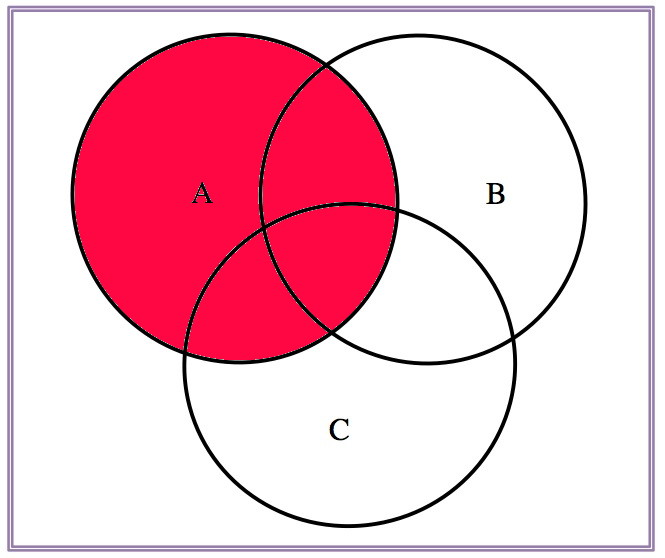
\includegraphics[width=\textwidth,height=2.08333in]{Images/proba1dibujos/distr11.jpg}
&
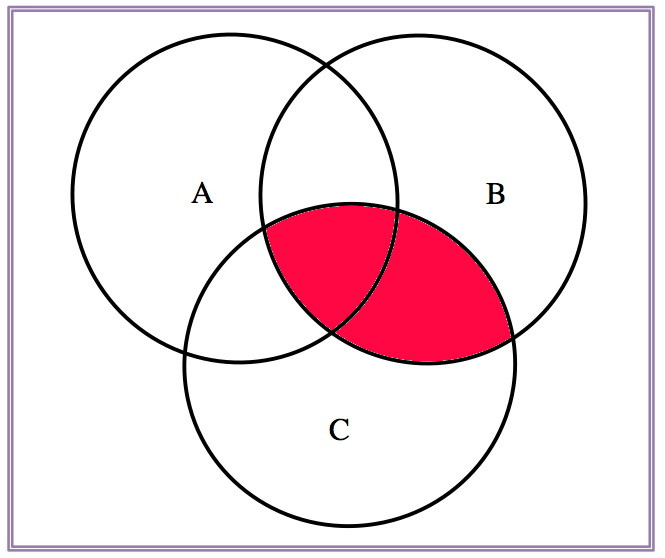
\includegraphics[width=\textwidth,height=2.08333in]{Images/proba1dibujos/distr12.jpg}
&
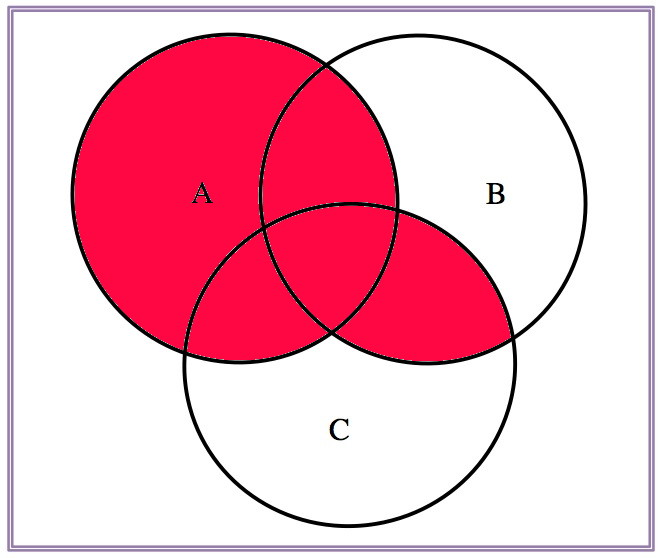
\includegraphics[width=\textwidth,height=2.08333in]{Images/proba1dibujos/distr13.jpg} \\
\bottomrule
\end{longtable}
\end{frame}

\begin{frame}{Propiedades}
\protect\hypertarget{propiedades-2}{}
\begin{longtable}[]{@{}ccc@{}}
\toprule
\(A\cup B\) & \(A\cup C\) & \((A\cup B)\cap (A\cup C)\) \\
\midrule
\endhead
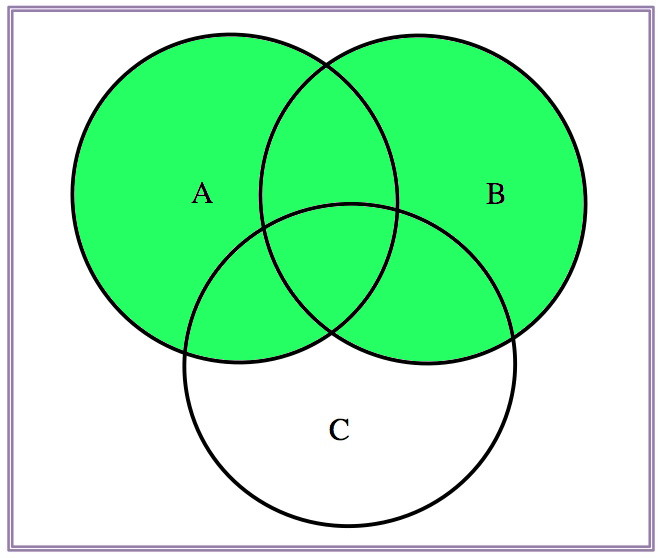
\includegraphics[width=\textwidth,height=2.08333in]{Images/proba1dibujos/distr21.jpg}
&
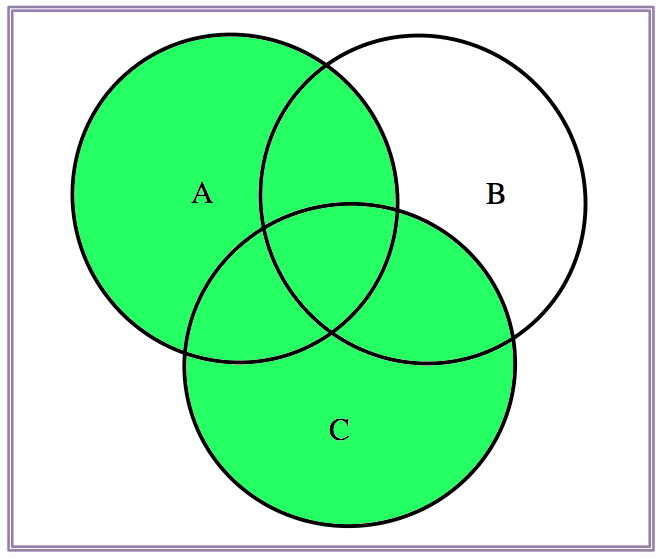
\includegraphics[width=\textwidth,height=2.08333in]{Images/proba1dibujos/distr22.jpg}
&
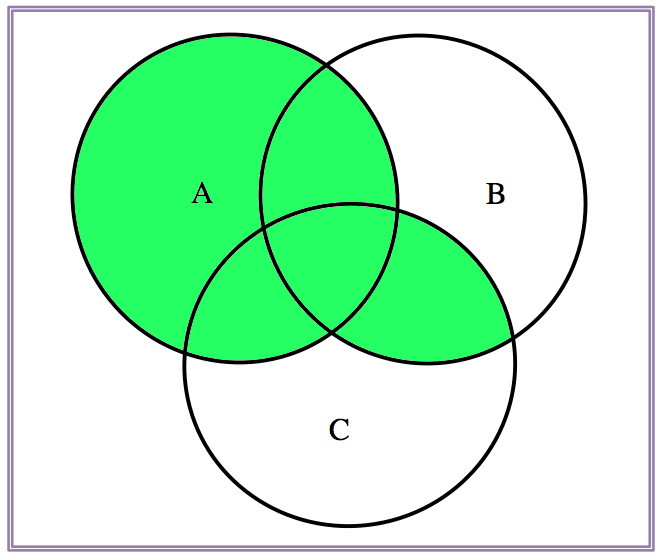
\includegraphics[width=\textwidth,height=2.08333in]{Images/proba1dibujos/distr23.jpg} \\
\bottomrule
\end{longtable}
\end{frame}

\begin{frame}{Propiedades}
\protect\hypertarget{propiedades-3}{}
Complementario del complementario \[(A^c)^c=A\]

\begin{longtable}[]{@{}ccc@{}}
\toprule
\(A\) & \(A^c\) & \((A^c)^c\) \\
\midrule
\endhead
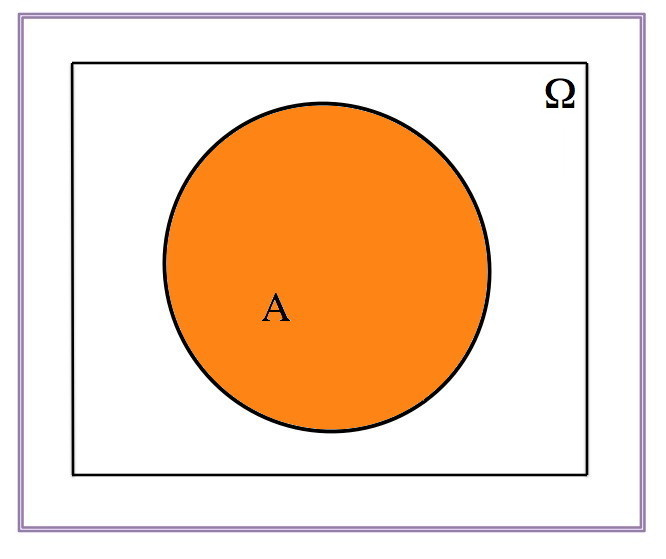
\includegraphics[width=\textwidth,height=2.08333in]{Images/proba1dibujos/dd2.jpg}
&
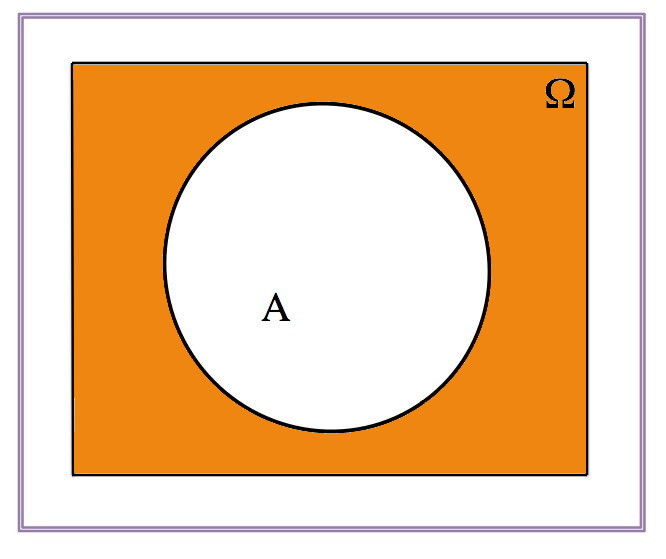
\includegraphics[width=\textwidth,height=2.08333in]{Images/proba1dibujos/dd1.jpg}
&
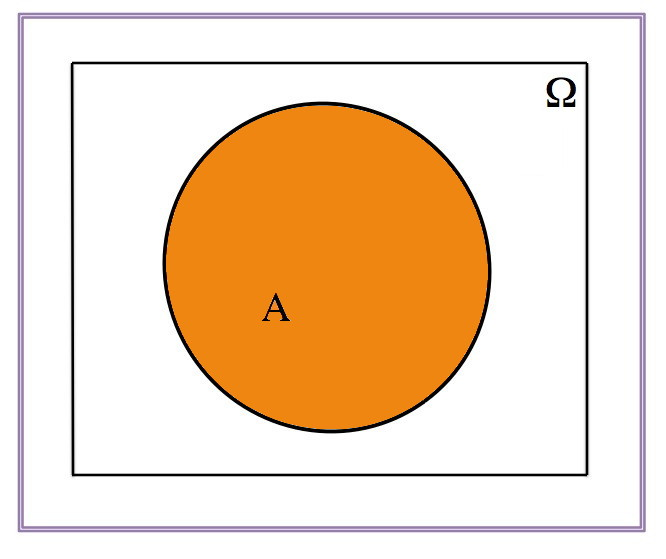
\includegraphics[width=\textwidth,height=2.08333in]{Images/proba1dibujos/dd3.jpg} \\
\bottomrule
\end{longtable}
\end{frame}

\begin{frame}{Propiedades}
\protect\hypertarget{propiedades-4}{}
Leyes de De Morgan

\[(A\cup B)^c=A^c\cap B^c\]

\begin{longtable}[]{@{}cc@{}}
\toprule
\(A\cup B\) & \((A\cup B)^c\) \\
\midrule
\endhead
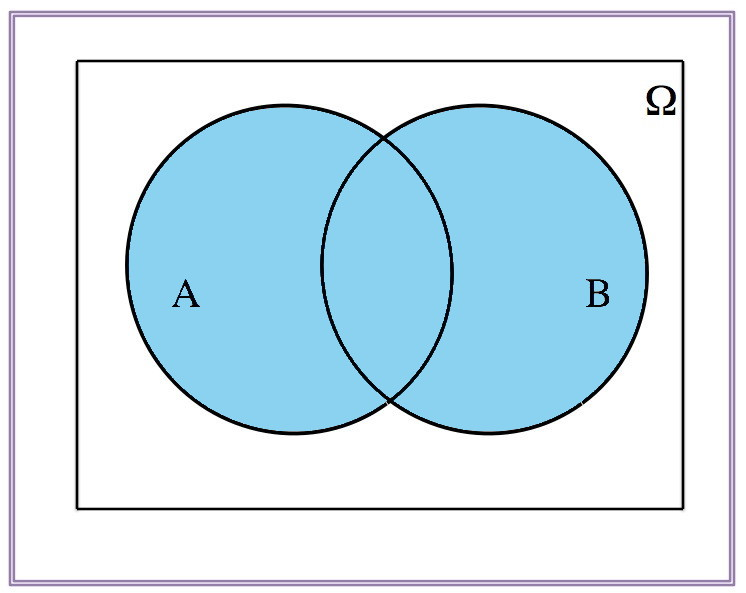
\includegraphics[width=\textwidth,height=2.08333in]{Images/proba1dibujos/demorgan6.jpg}
&
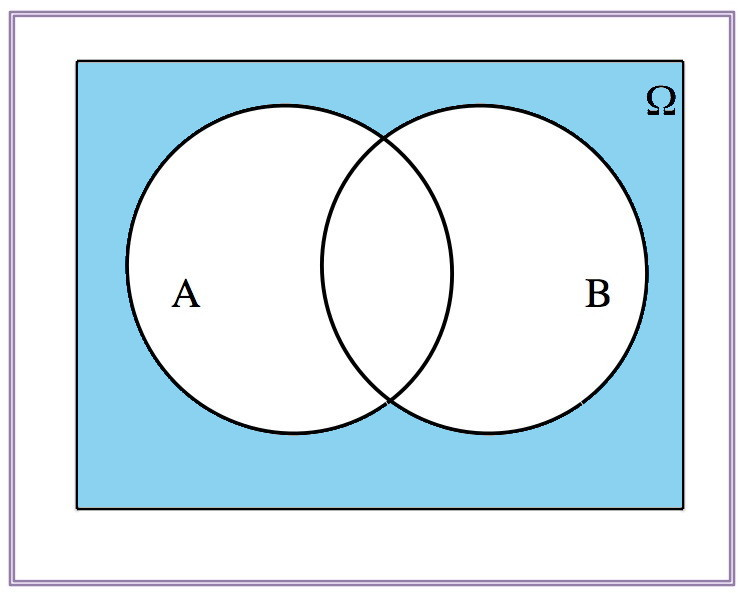
\includegraphics[width=\textwidth,height=2.08333in]{Images/proba1dibujos/demorgan7.jpg} \\
\bottomrule
\end{longtable}
\end{frame}

\begin{frame}{Propiedades}
\protect\hypertarget{propiedades-5}{}
Leyes de De Morgan

\[(A\cup B)^c=A^c\cap B^c\]

\begin{longtable}[]{@{}ccc@{}}
\toprule
\(A^c\) & \(B^c\) & \(A^c\cap B^c\) \\
\midrule
\endhead
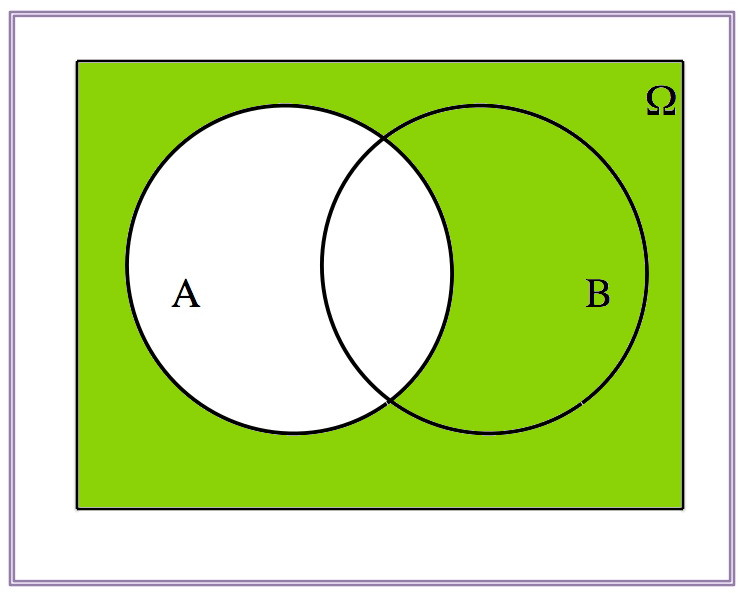
\includegraphics[width=\textwidth,height=2.08333in]{Images/proba1dibujos/demorgan8.jpg}
&
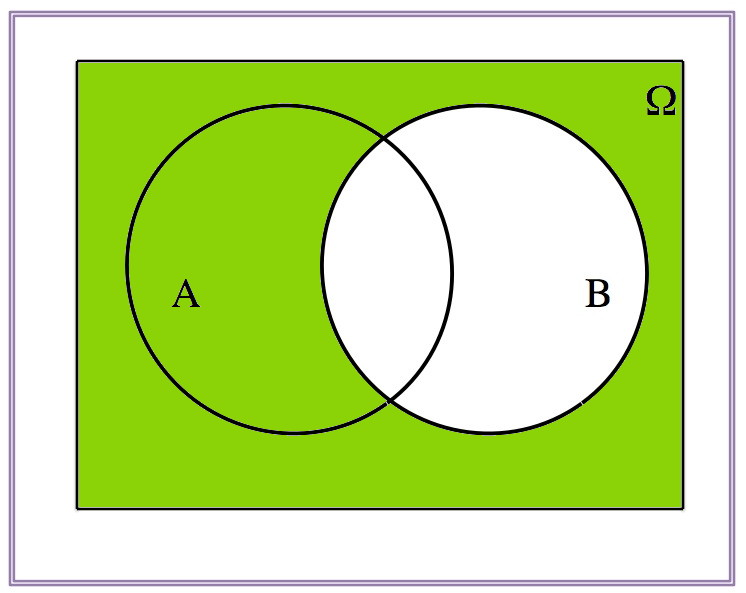
\includegraphics[width=\textwidth,height=2.08333in]{Images/proba1dibujos/demorgan9.jpg}
&
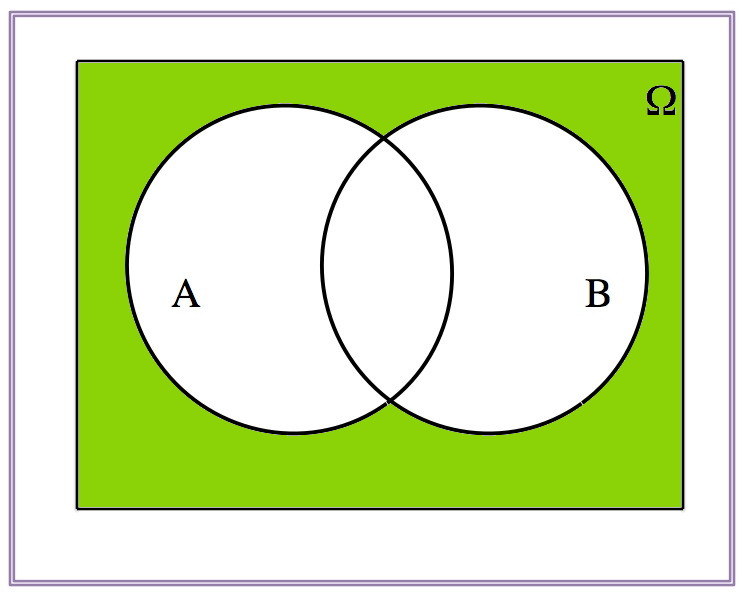
\includegraphics[width=\textwidth,height=2.08333in]{Images/proba1dibujos/demorgan10.jpg} \\
\bottomrule
\end{longtable}
\end{frame}

\begin{frame}{Propiedades}
\protect\hypertarget{propiedades-6}{}
Leyes de De Morgan

\[(A\cap B)^c=A^c\cup B^c\]

\begin{longtable}[]{@{}cc@{}}
\toprule
\(A\cap B\) & \((A\cap B)^c\) \\
\midrule
\endhead
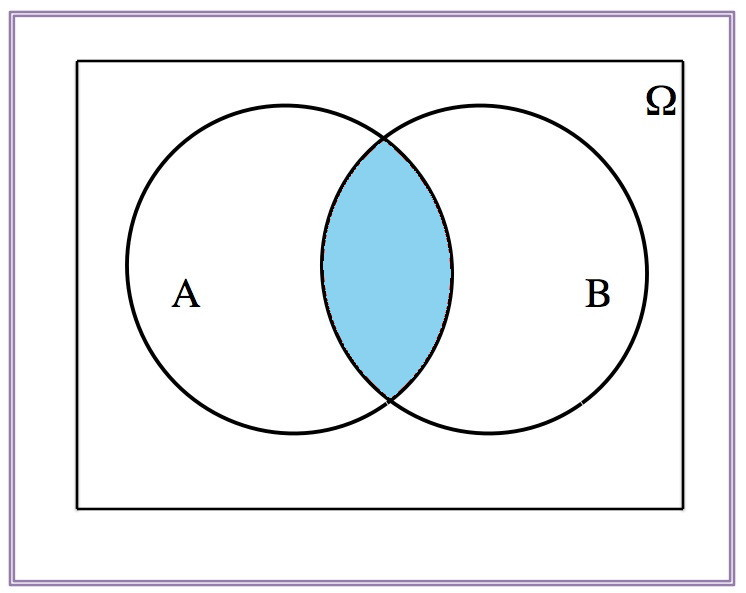
\includegraphics[width=\textwidth,height=2.08333in]{Images/proba1dibujos/demorgan1.jpg}
&
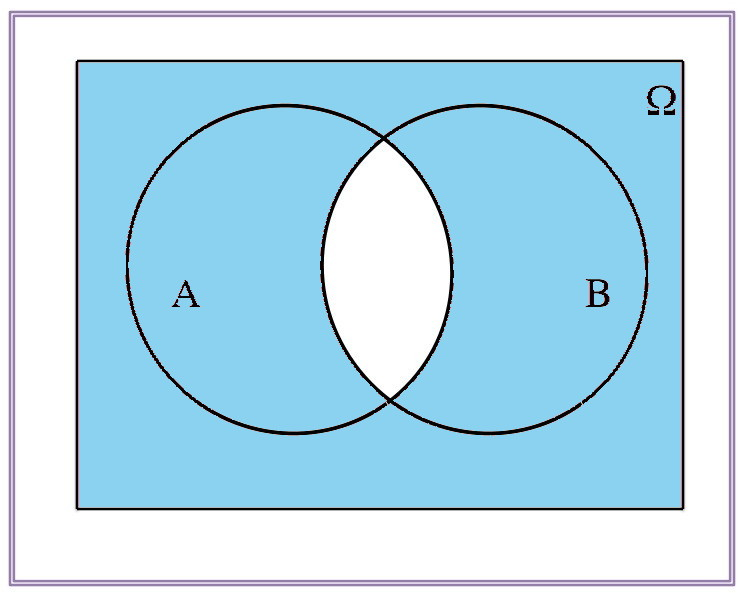
\includegraphics[width=\textwidth,height=2.08333in]{Images/proba1dibujos/demorgan2.jpg} \\
\bottomrule
\end{longtable}
\end{frame}

\begin{frame}{Propiedades}
\protect\hypertarget{propiedades-7}{}
Leyes de De Morgan

\[(A\cap B)^c=A^c\cup B^c\]

\begin{longtable}[]{@{}ccc@{}}
\toprule
\(A^c\) & \(B^c\) & \(A^c\cup B^c\) \\
\midrule
\endhead
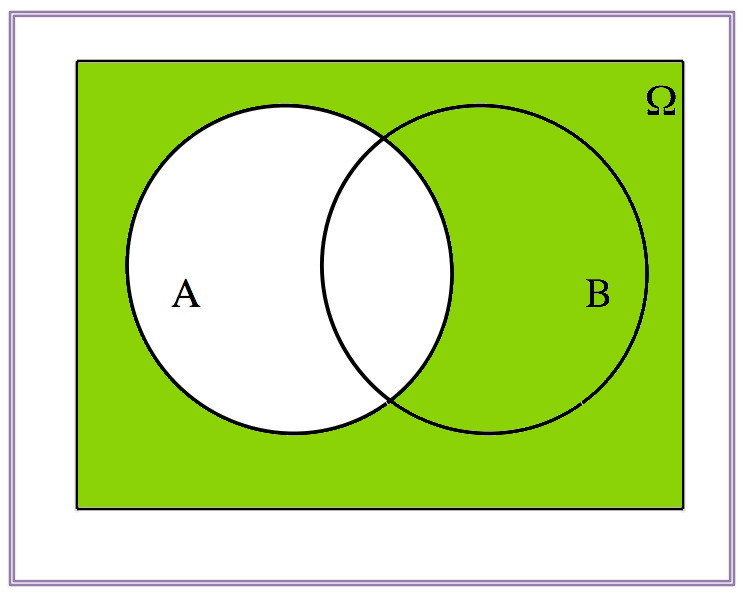
\includegraphics[width=\textwidth,height=2.08333in]{Images/proba1dibujos/demorgan3.jpg}
&
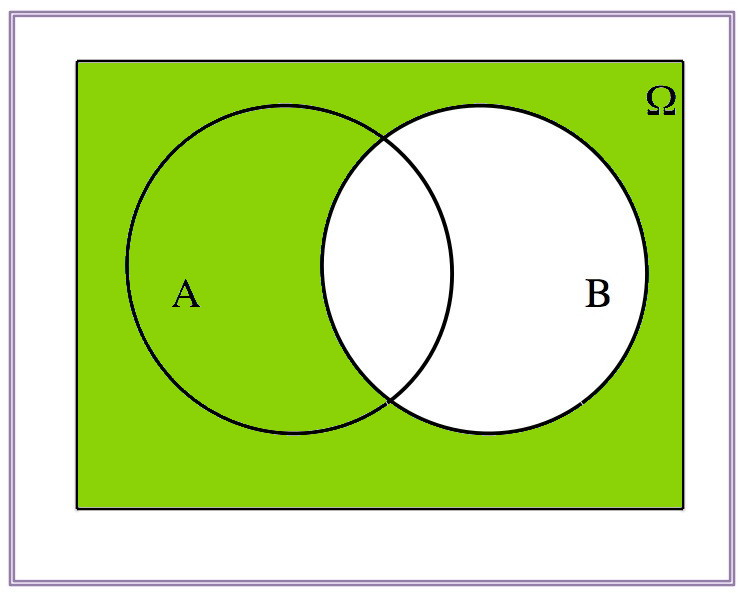
\includegraphics[width=\textwidth,height=2.08333in]{Images/proba1dibujos/demorgan5.jpg}
&
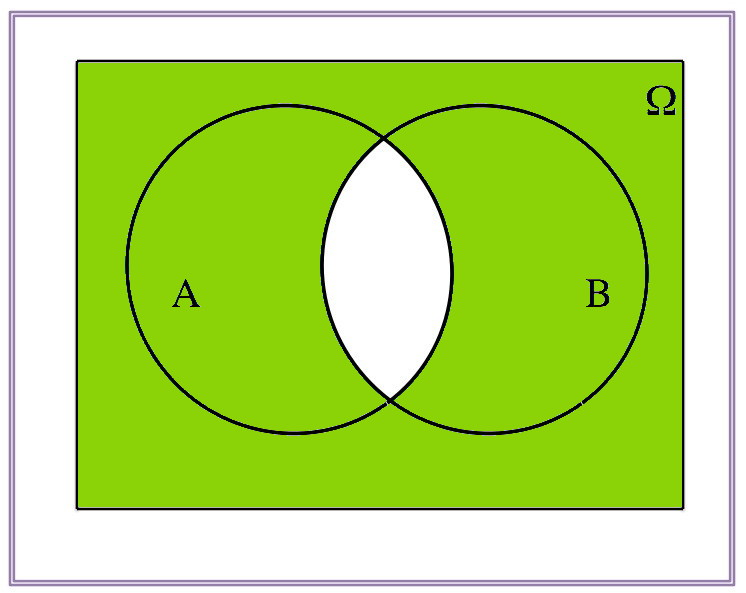
\includegraphics[width=\textwidth,height=2.08333in]{Images/proba1dibujos/demorgan4.jpg} \\
\bottomrule
\end{longtable}
\end{frame}

\begin{frame}{Definición de probabilidad}
\protect\hypertarget{definiciuxf3n-de-probabilidad}{}
La probabilidad de un suceso es una puntuación (\emph{score}) numérico
entre 0 y 1 que mide la verosimilitud de que este evento se produzca.

Esta verosimilitud puede estar justificada por:

\begin{itemize}
\item
  Estimación personal
\item
  Estimación de expertos
\item
  La frecuencia con la que se da
\item
  Cálculo formal
\end{itemize}
\end{frame}

\begin{frame}{Definición de probabilidad}
\protect\hypertarget{definiciuxf3n-de-probabilidad-1}{}
Definición formal de probabilidad

Sea \(\Omega\) el espacio muestral de un experimento aleatorio.
Supongamos que el número de posibles resultados, por el momento, es
finito.

Una probabilidad sobre \(\Omega\) es una aplicación
\(P:\mathcal{P}(\Omega)\to [0,1]\) con las siguientes propiedades:

\begin{enumerate}
\tightlist
\item
  \(0\leq P(A)\leq 1\), para todo suceso \(A\).
\item
  \(P(\Omega)=1\).
\item
  Si \(\{A_1,A_2,\ldots,A_n\}\) son sucesos disjuntos dos a dos,
  entonces
\end{enumerate}

\[
P(A_1\cup A_2\cup \cdots \cup A_n)=P(A_1)+P(A_2)+\cdots +P(A_n)
\]

Si \(a\in \Omega\) es un suceso elemental cometeremos el abuso de
notación de poner \(P(a)\) en lugar de \(P(\{a\})\)
\end{frame}

\begin{frame}{Ejemplo: grupos sanguíneos}
\protect\hypertarget{ejemplo-grupos-sanguuxedneos}{}
\textbf{Ejemplo}

En la página de la
\href{http://www.donasang.org/que-es-la-sang/es_frequencies-dels-diferents-grups.html}{Fundación
Banco de Sangre y Tejidos de las Islas Baleares} podemos encontrar
información sobre los porcentajes de tipos de sangre de los donantes de
las Islas Baleares:

\[A: 46\%;\  B: 7.5\%;\  AB: 3.5\%;\  O: 43\%.\]

¿Cuál es la probabilidad de que un balear donante de sangre no sea del
tipo O?

\textbf{Experimento aleatorio:} tipo de sangre de un paciente humano

\[\Omega=\{\mbox{A,B,AB,O}\}\]

\textbf{Probabilidad} de un suceso: se asimila al porcentaje observado
de individuos

\textbf{Suceso:} \(\{\mbox{O}\}^c=\{\mbox{A,B,AB}\}\)

\[P(\{\mbox{O}\}^c)\!=\!P(\{\mbox{A,B,AB}\})\!=\!
P(\mbox{A})+P (\mbox{B})+P(\mbox{AB})\!=\!0.57\]
\end{frame}

\begin{frame}{Propiedades}
\protect\hypertarget{propiedades-8}{}
Propiedades básicas de la probabilidad

\begin{itemize}
\item
  \(P(\emptyset)=0\).
\item
  \(P(A-B)=P(A)-P(A\cap B)\) porque \(P(A)=P(A-B)+P(A\cap B)\).
\end{itemize}

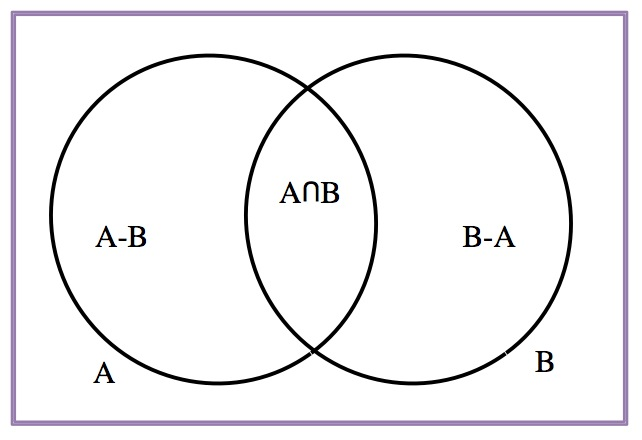
\includegraphics[width=\textwidth,height=2.08333in]{Images/proba1dibujos/A-B.jpg}

\begin{itemize}
\item
  Si \(B\subseteq A\), entonces \(0\leq P(B)\leq P(A)\).
\item
  \(P(A^c)=1-P(A)\).
\end{itemize}
\end{frame}

\begin{frame}{Propiedades}
\protect\hypertarget{propiedades-9}{}
\begin{itemize}
\tightlist
\item
  \(P(A\cup B)=P(A)+P(B)-P(A\cap B)\) porque
\end{itemize}

\[\begin{eqnarray*}
P(A)+P(B)-P(A\cap B) &=& P(A-B)+P(A\cap B)+\\
 & & P(B-A)+ P(A\cap  B)-P(A\cap  B)\\
&=& P(A-B)+P(A\cap B)+ P(B-A) \\
&=& P(A\cup B).
\end{eqnarray*}\]

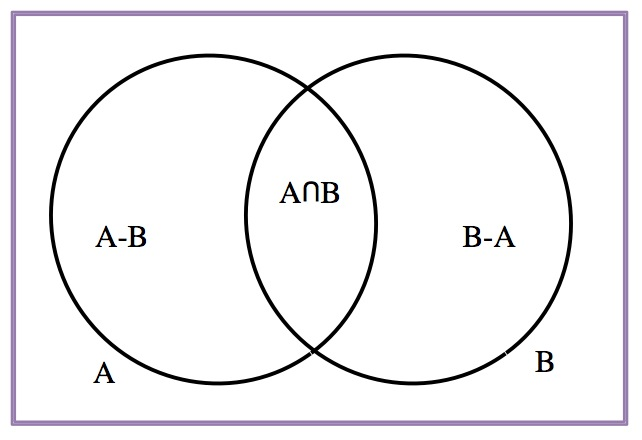
\includegraphics[width=\textwidth,height=2.08333in]{Images/proba1dibujos/A-B.jpg}
\end{frame}

\begin{frame}{Propiedades}
\protect\hypertarget{propiedades-10}{}
\begin{itemize}
\tightlist
\item
  \[\begin{eqnarray*}
  P(A\cup B\cup C)&=&P(A)+P(B)+P(C)  \\ &&-P(A\cap B)-P(A\cap C)-P(B\cap C)  +P(A\cap B\cap C)
  \end{eqnarray*}\]
\end{itemize}

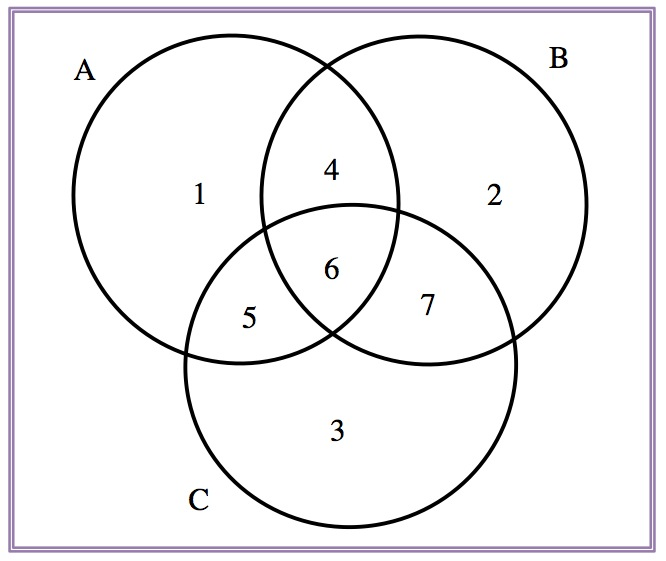
\includegraphics[width=\textwidth,height=2.08333in]{Images/proba1dibujos/tresconjunts.jpg}

\[P(A\cup B\cup C)=P(1)+P(2)+P(3)+P(4)+P(5)+P(6)+P(7).\]
\end{frame}

\begin{frame}{Propiedades}
\protect\hypertarget{propiedades-11}{}
\begin{itemize}
\item
  Si \(A=\{a_1,a_2,\ldots,a_k\}\), entonces \[
  P(A)=P(a_1)+P(a_2)+\cdots+P(a_k).
  \]
\item
  Si todos los sucesos elementales tienen la misma probabilidad, \[
  P(A)=\frac{|A|}{|\Omega|}\Big(=\frac{\mbox{casos favorables}}{\mbox{casos posibles}}\Big).
  \]
\end{itemize}
\end{frame}

\begin{frame}{Ejemplo: Frecuencia de vocales}
\protect\hypertarget{ejemplo-frecuencia-de-vocales}{}
\textbf{Ejemplo}

Los porcentajes de vocales de un determinado idioma (de alfabeto latino)
según la
\href{https://es.wikipedia.org/wiki/Frecuencia_de_aparici\%C3\%B3n_de_letras}{Wikipedia}
son:

\[A: 18.7\%;\ E: 26.1\%;\ I: 25.7\%;\ O: 24.4\%;\ U: 5.1\%.\]

¿Cuál es la probabilidad que una vocal escogida al azar de este idioma
sea una E o una O?

El espacio muestral del experimento es \(\Omega=\{A,E,I,O,U\}\).

El suceso que deseamos analizar es \(\{E,0\}\).

Y su probabilidad es

\[P(\{E,O\})=P(E)+P(O)=0.261+0.244=0.505.\]
\end{frame}

\begin{frame}{Ejemplo: Consumo de drogas}
\protect\hypertarget{ejemplo-consumo-de-drogas}{}
Segun un árticulo de
\href{https://elpais.com/politica/2019/01/02/actualidad/1546426491_623324.html}{El
País}, en un control especial de la policía el \(0.1\%\) de todos los
conductores analizados en un control de tráfico dan positivo en un el
test en cocaína, y el \(1\%\) da positivo en cannabis. Un \(1.05\%\) da
positivo en alguno de los dos test.

¿Cuál es la probabilidad que un individuo analizado en el control de
drogas escogido al azar no de positivo en ninguno de lo dos test?

Los sucesos elementales del enunciado del problema son:

\begin{itemize}
\tightlist
\item
  \(A\): dar positivo en cocaína; \(P(A)=0.001.\)
\item
  \(B\): dar positivo en cannabis; \(P(B)=0.01.\)
\end{itemize}

En este caso nos interesa estudiar los sucesos:

\begin{itemize}
\tightlist
\item
  \(A\cup B\): dar positivo en alguno de los dos test;
  \(P(A\cup B)=0.0105.\)
\item
  \((A\cup B)^c\): no dar positivo en ninguno de los test,
\end{itemize}

por tanto: \[P((A\cup B)^c)=1-P(A\cup B)=1-0.0105=0.9895.\]
\end{frame}

\begin{frame}{Ejemplos: Consumo de drogas}
\protect\hypertarget{ejemplos-consumo-de-drogas}{}
\textbf{Ejemplo}

En un control especial de la policía el \(0.1\%\) de todos los
conductores analizados en un control de tráfico dan positivo en un el
test en cocaína, y el \(1\%\) da positivo en cannabis. Un \(1.05\%\) da
positivo en alguno de los dos test.

¿Cuál es la probabilidad que un analizado al azar de positivo en los dos
test en cocaína y cannabis?

Los sucesos elementales son:

\begin{itemize}
\tightlist
\item
  \(A\): dar positivo en cocaína; \(P(A)=0.001.\)
\item
  \(B\): dar positivo en cannabis; \(P(B)=0.01.\)
\end{itemize}

En este caso nos interesa estudiar los sucesos:

\begin{itemize}
\tightlist
\item
  \(A\cup B\): dar positivo en algún de los dos test;
  \(P(A\cup B)=0.0105.\)
\item
  \(A\cap B\): dar positivo en los dos test
\end{itemize}

de donde, por tanto:

\[\begin{array}{rl}
{P(A\cap B)} &{=P(A)+P(B)-P(A\cup B)}\\ &{=0.001+0.01-0.0105=0.0005}.
\end{array}\]
\end{frame}

\begin{frame}{Ejemplo: Control de drogas}
\protect\hypertarget{ejemplo-control-de-drogas}{}
\textbf{Ejemplo}

En un control especial de la policía el \(0.1\%\) de todos los
conductores analizados en un control de tráfico dan positivo en un el
test en cocaína, y el \(1\%\) da positivo en cannabis. Un \(1.05\%\) da
positivo en alguno de los dos test.

¿Cuál es la probabilidad de que un conductor analizado de positivo en
cocaína pero no en cannabis?

Los sucesos elementales son:

\begin{itemize}
\tightlist
\item
  \(A\): dar positivo en cocaína; \(P(A)=0.001.\)
\item
  \(B\): dar positivo en cannabis; \(P(B)=0.01.\)
\end{itemize}

En este caso nos interesa estudiar los sucesos:

\begin{itemize}
\tightlist
\item
  \(A\cap B\): dar positivo en los dos test; \(P(A\cap B)=0.0005.\)
\item
  \(A-B\): dar positivo en cocaína pero no en cannabis,
\end{itemize}

de donde, por tanto:

\[P(A-B) =P(A)-P(A\cap B) =0.001-0.0005=0.0005.\]
\end{frame}

\hypertarget{probabilidad-condicionada}{%
\section{Probabilidad condicionada}\label{probabilidad-condicionada}}

\begin{frame}{Probabilidad condicionada}
\protect\hypertarget{probabilidad-condicionada-1}{}
Probabilidad condicionada: Dados dos sucesos \(A\) y \(B\), con
\(P(A)>0\), la probabilidad \(P(B|A)\) de \(B\) condicionado a \(A\) es
la probabilidad

\begin{itemize}
\tightlist
\item
  de que suceda \(B\) suponiendo que pasa \(A\),
\item
  de que si pasa \(A\), entonces suceda \(B\),
\item
  de que un resultado de \(A\) también pertenezca a \(B\).
\end{itemize}

Se calcula a través de la definición:

\[
P(B|A)=\frac{P(A\cap B)}{P(A)}.
\]
\end{frame}

\begin{frame}{Ejemplo: frecuencia género y gafas}
\protect\hypertarget{ejemplo-frecuencia-guxe9nero-y-gafas}{}
\textbf{Ejemplo}

En una clase de 20 hombres y 30 mujeres, 15 hombres y 18 mujeres llevan
gafas. Contestemos las siguientes preguntas:

\begin{itemize}
\tightlist
\item
  ¿Cuál es la probabilidad de que un alumno lleve gafas?
\end{itemize}

\[
\frac{33}{50}
\]

\begin{itemize}
\tightlist
\item
  ¿Cuál es la probabilidad de que un alumno sea mujer y lleve gafas?
\end{itemize}

\[
\frac{18}{50}
\]
\end{frame}

\begin{frame}{Ejemplo: sexo y gafas}
\protect\hypertarget{ejemplo-sexo-y-gafas}{}
\textbf{Ejemplo}

En una clase de 20 hombres y 30 mujeres, 15 hombres y 18 mujeres llevan
gafas. Contestemos las siguientes preguntas:

\begin{itemize}
\tightlist
\item
  ¿Cuál es la probabilidad de que un chica lleve gafas?
\end{itemize}

\[
\frac{18}{30}=\frac{18/50}{30/50}=\frac{P(\mbox{mujer  y gafas})}{P(\mbox{mujer})}.
\]

\begin{itemize}
\tightlist
\item
  Si escogemos un estudiante al azar ¿Cuál es la probabilidad que si es
  mujer, entonces lleve gafas?
\end{itemize}

\[
\frac{18}{30}.
\]
\end{frame}

\begin{frame}{Ejemplo}
\protect\hypertarget{ejemplo}{}
\textbf{Ejemplo}

En una clase de 20 hombres y 30 mujeres, 15 hombres y 18 mujeres llevan
gafas. Contestemos las siguientes preguntas:

\begin{itemize}
\tightlist
\item
  ¿Cuál es la probabilidad de que un alumno que lleve gafas sea mujer?
\end{itemize}

\[
\frac{18}{33}=\frac{18/50}{33/50}=\frac{P(\mbox{mujer y gafas})}{P(\mbox{gafas})}.
\]

\begin{itemize}
\tightlist
\item
  Si escogemos un estudiante al azar ¿Cuál es la probabilidad de que si
  lleva gafas, entonces sea mujer? \[
  \frac{18}{33}
  \]
\end{itemize}
\end{frame}

\begin{frame}{¡Atención!}
\protect\hypertarget{atenciuxf3n}{}
Hay que distinguir bien entre

\begin{itemize}
\tightlist
\item
  \(P(A\cap B)\): probabilidad de \(A\) \(\color{red}{\text{y}}\) \(B\).
\end{itemize}

\emph{Probabilidad de que sea mujer y lleve gafas.}

\begin{itemize}
\tightlist
\item
  \(P(A|B)\): probabilidad de que \(\color{red}{\text{si}}\) pasa \(B\),
  \(\color{red}{\text{entonces}}\) pase \(A\).
\end{itemize}

\emph{Probabilidad de que, si es mujer, lleve gafas.}

Cuando utilizamos probabilidad condicional \(P(A|B)\) estamos
restringiendo el espacio muestral a \(B\).
\end{frame}

\begin{frame}{Probabilidad condicionada. Propiedades}
\protect\hypertarget{probabilidad-condicionada.-propiedades}{}
La probabilidad condicionada es una probabilidad

Proposición

Sea \(A\subseteq \Omega\) un suceso tal que \(P(A)>0\), entonces

\[
\begin{array}{rccl}
P(-|A):& \mathcal{P}(\Omega) & \to & [0,1]\\
&B & \mapsto & P(B|A).
\end{array}
\] satisface las propiedades de las probabilidades, como por ejemplo:

\[
\begin{array}{l}
P(B^c|A)=1-P(B|A),\\
P(B_1\cup B_2|A)=P(B_1|A)+P(B_2|A)-P(B_1\cap B_2|A).
\end{array}
\]

\textbf{Ejercicio}

Escribid el resto de propiedades que cumpliría una probabilidad
condicionada al evento \(A\).
\end{frame}

\begin{frame}{Ejemplos}
\protect\hypertarget{ejemplos}{}
\textbf{Ejemplo}

Un 15\% de los adultos son hipertensos, un 25\% de los adultos creen que
son hipertensos, y un 9\% de los adultos son hipertensos y creen que lo
son.

Si un adulto cree que es hipertenso, ¿cuál es la probabilidad que lo
sea?

Sean los sucesos

\begin{itemize}
\tightlist
\item
  \(A\): ser hipertenso, \(P(A)=0.15\) ,
\item
  \(B\): creer ser hipertenso, \(P(B)=0.25\),
\end{itemize}

entonces podemos definir el suceso:

\begin{itemize}
\tightlist
\item
  \(A\cap B\): ser hipertenso y creerlo, \(P(A\cap B)=0.09\).
\end{itemize}

de donde, la probabilidad condicionada de ser hipertenso creyéndonos que
lo somos es:

\[P(A|B)=\dfrac{P(A\cap B)}{P(B)}=\dfrac{0.09}{0.25}=0.36.\]
\end{frame}

\begin{frame}{Ejemplo}
\protect\hypertarget{ejemplo-1}{}
\textbf{Ejemplo}

Un 15\% de los adultos son hipertensos, un 25\% de los adultos creen que
son hipertensos, y un 9\% de los adultos son hipertensos y creen que lo
son.

Si un adulto es hipertenso, ¿cuál es la probabilidad que crea que lo es?

Si tenemos los sucesos:

\begin{itemize}
\tightlist
\item
  \(A\): ser hipertenso,
\item
  \(B\): creer ser hipertenso
\end{itemize}

entonces buscamos la probabilidad \(P(B|A)\):

\[
\begin{array}{rl}
P(B|A) & =\dfrac{P(A\cap B)}{P(A)}=\dfrac{0.09}{0.15}=
0.6
\end{array}
\]
\end{frame}

\begin{frame}{Ejemplos: dígitos de control}
\protect\hypertarget{ejemplos-duxedgitos-de-control}{}
\textbf{Ejemplo}

Un dígito de control de error toma el valor 0 en el 99\% de los casos en
que hay un error. Si la probabilidad de error en un mensaje es del
\(0.5\%\). ¿cuál es la probabilidad de que el mensaje sea erróneo y el
código de error tenga valor 0?

\begin{itemize}
\tightlist
\item
  \(B\): mensaje con error; \(P(B)=0.005\),
\item
  \(A\): código de error vale 0,
\item
  \(P(A|B)=0.99\),
\end{itemize}

entonces: \[P(A\cap B)=P(B)\cdot P(A|B)=0.005\cdot 0.99=0.00495.\]
\end{frame}

\begin{frame}{Ejemplos}
\protect\hypertarget{ejemplos-1}{}
\textbf{Ejemplo: SPAM}

Un 50\% de correos recibidos en un servidor llevan adjuntos y un 65\%
son publicidad no deseada (SPAM). Sólo un 15\% de estos correos no
llevan adjuntos y no son SPAM.

\begin{itemize}
\tightlist
\item
  ¿Cuál es la probabilidad que un correo lleve adjunto si es SPAM?
\item
  ¿Cuál es la probabilidad que un correo \textbf{no} tenga adjuntos si
  \textbf{no} es SPAM?
\end{itemize}
\end{frame}

\begin{frame}{Ejemplos}
\protect\hypertarget{ejemplos-2}{}
\textbf{Ejemplo}

Un 50\% de correos recibidos en un servidor llevan adjuntos y un 65\%
son publicidad no deseada (SPAM). Sólo un 15\% de estos correos no
llevan adjuntos y no son SPAM.

\begin{itemize}
\tightlist
\item
  ¿Cuál es la probabilidad que un correo lleve adjunto si es SPAM?
\end{itemize}

\begin{itemize}
\tightlist
\item
  \(A\): llevar adjuntos; \(P(A)=0.5\),
\item
  \(S\): SPAM; \(P(S)=0.65\),
\item
  \(A^c\cap S^c=(A\cup S)^c\): no llevar adjunto y no ser SPAM;
  \(P((A\cup S)^c)=0.15\),
\end{itemize}

\[P(A|S)=\dfrac{P(A\cap S)}{P(S)}=?\]
\end{frame}

\begin{frame}{Ejemplos}
\protect\hypertarget{ejemplos-3}{}
\textbf{Ejemplo}

Un 50\% de correos recibidos en un servidor llevan adjuntos y un 65\%
son publicidad no deseada (SPAM). Sólo un 15\% de estos correos no
llevan adjuntos y no son SPAM.

\begin{itemize}
\tightlist
\item
  ¿Cuál es la probabilidad que un correo lleve adjunto si es SPAM?
\end{itemize}

\begin{itemize}
\item
  \(P(A)=0.5, P(S)=0.65, P(A^c\cap S^c)=P((A\cup S)^c)=0.15\),
\item
  \(P(A\cup S)=1-P((A\cup S)^c)=0.85\),
\item
  \(P(A\cap S)=P(A)+P(S)-P(A\cup S)=0.3\),
\end{itemize}

\[P(A|S)=\dfrac{P(A\cap S)}{P(S)}=\dfrac{0.3}{0.65}\approx 0.46.\]
\end{frame}

\begin{frame}{Ejemplos SPAM continuación}
\protect\hypertarget{ejemplos-spam-continuaciuxf3n}{}
\textbf{Ejemplo}

Un 50\% de correos recibidos en un servidor llevan adjuntos y un 65\%
son publicidad no deseada (SPAM). Sólo un 15\% de estos correos no
llevan adjuntos y no son SPAM.

\begin{itemize}
\tightlist
\item
  ¿Cuál es la probabilidad de que un correo no lleve adjuntos si no es
  SPAM?
\end{itemize}

\begin{itemize}
\tightlist
\item
  \(P(A)=0.5, P(S)=0.65, P(A^c\cap S^c)=P((A\cup S)^c)=0.15.\)
\end{itemize}

\[P(A^c|S^c)=\dfrac{P(A^c\cap S^c)}{P(S^c)}=\dfrac{P(A^c\cap S^c)}{1-P(S)}=\dfrac{0.15}{0.35}\approx 0.43.\]
\end{frame}

\begin{frame}{Teorema de la probabilidad total}
\protect\hypertarget{teorema-de-la-probabilidad-total}{}
Teorema de la probabilidad total

Dados dos sucesos \(A\) y \(B\) se tiene que

\[
\begin{array}{rl}
P(B)&= P(B\cap A) +P(B\cap A^c)\\
& =P(A)\cdot P(B|A)+ P(A^c)\cdot P(B|A^c).
\end{array}
\]
\end{frame}

\begin{frame}{Teorema de la probabilidad total}
\protect\hypertarget{teorema-de-la-probabilidad-total-1}{}
Partición del espacio espacio muestral

Los sucesos \(A_1,A_2,\ldots, A_n\) son una \textbf{partición} del
espacio muestral \(\Omega\) de un determinado experimento aleatorio, si
cumplen las condiciones siguientes:

\begin{enumerate}
\tightlist
\item
  \(A_1\cup A_2\cup\ldots\cup A_n=\Omega\),
\item
  \(A_1,A_2,\ldots,A_n\) son incompatibles dos a dos
  (\(A_i\cap A_j=\emptyset\)).
\end{enumerate}

Teorema de la probabilidad total

Sea \(A_1,A_2,\ldots,A_n\) una partición de \(\Omega\). Sea \(B\) un
suceso cualquiera. Entonces

\[
\begin{array}{rl}
P(B)&= P(B\cap A_1)+\cdots +P(B\cap A_n)\\
& =P(A_1)\cdot P(B|A_1)+\ldots+P(A_n)\cdot P(B|A_n).
\end{array}
\]
\end{frame}

\begin{frame}{Ejemplos}
\protect\hypertarget{ejemplos-4}{}
\textbf{Ejemplo}

Un dígito de control de error toma el valor 0 en un \(99\%\) de los
casos en que hay un error y en un \(5\%\) de los mensajes sin error. La
probabilidad de error en un mensaje es del \(0.5\%\).

¿Cuál es la probabilidad de que un mensaje escogido al azar tenga el
dígito de control a 0?

Sean los sucesos del enunciado:

\begin{itemize}
\tightlist
\item
  \(B\): mensaje con error; \(P(B)=0.005\),
\item
  \(A\): código de error vale 0,
\end{itemize}

entonces obtenemos las probabilidades a partir del enunciado:

\begin{itemize}
\tightlist
\item
  \(P(A|B)=0.99,\)
\item
  \(P(A|B^c)= 0.0,5\)
\end{itemize}

y por tanto,

\[
\begin{array}{rl}
P(A) & =P(B)\cdot P(A|B)+P(B^c)\cdot P(A|B^c)\\ &
=0.005\cdot 0.99+0.995\cdot 0.05=0.0547.
\end{array}
\]
\end{frame}

\begin{frame}{Clasificación o Diagnósticos}
\protect\hypertarget{clasificaciuxf3n-o-diagnuxf3sticos}{}
Consideremos alguna de las siguientes situaciones:

\begin{itemize}
\tightlist
\item
  Un algoritmo detecta si una transacción con tarjeta de crédito es
  fraude o no.
\item
  Un algoritmo detecta si tiene o no que mostrar un anuncio en una web.
\item
  Un prueba de embarazo.
\item
  Una prueba médica para una enfermedad concreta.
\end{itemize}

Nos ceñiremos a la casuística más elemental el algoritmo de
clasificación o la diagnosis solo da dos resultado \textbf{Positivo} (sí
tienes la enfermedad, sí es un fraude) o \textbf{Negativo} (en caso
contrario).
\end{frame}

\begin{frame}{Clasificación o Diagnósticos}
\protect\hypertarget{clasificaciuxf3n-o-diagnuxf3sticos-1}{}
En todas estas situaciones podemos calcular lo que se llama
\textbf{matriz de confusión} que representa todas las situaciones
posibles. En el caso de estudiar una condición de tipo binario,

\begin{longtable}[]{@{}lcc@{}}
\toprule
& El Test da Positivo & El Test da Negativo \\
\midrule
\endhead
Condición Positiva & Correcto & Error \\
Condición Negativa & Error & Correcto \\
\bottomrule
\end{longtable}
\end{frame}

\begin{frame}{Clasificación o Diagnósticos}
\protect\hypertarget{clasificaciuxf3n-o-diagnuxf3sticos-2}{}
En general los modelos y algoritmos de clasificación suelen aportar
puntuaciones (\emph{scores}) que determinan el grado de pertenencia a
una clase, o que miden si dos objetos están en la misma clase.

Así el resultado del clasificador o del diagnóstico puede ser:

\begin{itemize}
\tightlist
\item
  \textbf{un número real}, en cuyo caso debe clasificador entre cada
  clase debe determinarse por un valor umbral (\emph{threshold}) por
  ejemplo para determinar si una persona está estresado podemos dar un
  \emph{scores} entre 0 y 1 (1 máximo estrés 0 estrés nulo),
\item
  \textbf{un resultado discreto} que indica directamente una de las
  clases (esto es necesario si es un algoritmo que debe decidir qué
  hacer con el objeto.
\end{itemize}
\end{frame}

\begin{frame}{Clasificación o Diagnósticos}
\protect\hypertarget{clasificaciuxf3n-o-diagnuxf3sticos-3}{}
\href{https://www.youtube.com/watch?v=pqTntG1RXSY}{\includegraphics{https://img.youtube.com/vi/pqTntG1RXSY/0.jpg}}
\end{frame}

\begin{frame}{Clasificación o Diagnósticos}
\protect\hypertarget{clasificaciuxf3n-o-diagnuxf3sticos-4}{}
Positivos y Negativos en Clasificación Consideremos un problema de
predicción de clases binario, en la que los resultados se etiquetan
positivos (P) o negativos (N). Hay cuatro posibles resultados a partir
de un clasificador binario como el propuesto.

\begin{itemize}
\tightlist
\item
  Si el resultado de una exploración es P y el valor dado es también P,
  entonces se conoce como un Verdadero Positivo (VP).
\item
  Sin embargo si el valor real es N entonces se conoce como un Falso
  Positivo (FP).
\item
  De igual modo, tenemos un Verdadero Negativo (VN) cuando tanto la
  exploración como el valor dado son N.
\item
  Un Falso Negativo (FN) cuando el resultado de la predicción es N pero
  el valor real es P.
\end{itemize}
\end{frame}

\begin{frame}{Clasificación o Diagnósticos}
\protect\hypertarget{clasificaciuxf3n-o-diagnuxf3sticos-5}{}
Un ejemplo aproximado de un problema real es el siguiente: consideremos
una prueba diagnóstica que persiga determinar si una persona tiene una
cierta enfermedad.

\begin{itemize}
\tightlist
\item
  Un falso positivo en este caso ocurre cuando la prueba predice que el
  resultado es positivo, cuando la persona no tiene realmente la
  enfermedad.
\item
  Un falso negativo, por el contrario, ocurre cuando el resultado de la
  prueba es negativo, sugiriendo que no tiene la enfermedad cuando
  realmente sí la tiene.
\end{itemize}
\end{frame}

\begin{frame}{Clasificación o Diagnósticos}
\protect\hypertarget{clasificaciuxf3n-o-diagnuxf3sticos-6}{}
En un diagnósticos de una cierta condición (por ejemplo, test embarazo,
test de enfermedad), tenemos dos tipos de sucesos:

\begin{itemize}
\tightlist
\item
  \(T\): el test da positivo,
\item
  \(M\): el sujeto satisface la condición.
\end{itemize}

Falsos Positivos y Falsos Negativos

\begin{itemize}
\tightlist
\item
  \textbf{Falsos positivos} \(T\cap M^c\): El test da positivo, pero la
  condición no se da,
\item
  \textbf{Coeficiente de falsos positivos} \(P(T|M^c)\),
\item
  \textbf{Falsos negativos} \(T^c\cap M\): El test da negativo, pero la
  condición sí que se da,
\item
  \textbf{Coeficiente de falsos negativos}: \(P(T^c|M)\).
\end{itemize}
\end{frame}

\begin{frame}{Clasificación o Diagnósticos}
\protect\hypertarget{clasificaciuxf3n-o-diagnuxf3sticos-7}{}
\textbf{Ejemplo}

Un test diseñado para diagnosticar una determinada enfermedad tiene un
coeficiente de falsos negativos de 0.06, y un coeficiente de falsos
positivos de 0.04. En un estudio masivo se observa que un 15\% de la
población da positivo al test.

¿Cuál es la probabilidad que una persona escogida aleatoriamente tenga
esta enfermedad?

Los datos del problema son:

\begin{itemize}
\tightlist
\item
  \(T\): dar positivo al test; \(P(T)=0.15\),
\item
  \(M\): tener la enfermedad,
\item
  \(P(T)=0.15\), \(P(T^c|M)=0.06\), \(P(T|M^c)=0.04\),
\item
  ¿\(P(M)\)?
\end{itemize}
\end{frame}

\begin{frame}{Ejemplos}
\protect\hypertarget{ejemplos-5}{}
\begin{itemize}
\tightlist
\item
  \(P(T)=0.15\), \(P(T^c|M)=0.06\), \(P(T|M^c)=0.04.\)
\end{itemize}

\[
P(T) =P(M)\cdot P(T|M)+P(M^c)\cdot P(T|M^c).
\]

donde

\[
\begin{array}{l}
P(T|M)=1-P(T^c|M)=0.94 \\
P(M^c)=1-P(M).
\end{array}
\]

Por lo tanto

\[
\begin{array}{rl}
0.15 & = P(M)\cdot 0.94+(1-P(M))\cdot 0.04\\
 & =0.04+0.9\cdot P(M)\\
P(M) & =\dfrac{0.11}{0.9}\approx 0.1222.
\end{array}
\]
\end{frame}

\hypertarget{bayes}{%
\section{Bayes}\label{bayes}}

\begin{frame}{Fórmula de Bayes}
\protect\hypertarget{fuxf3rmula-de-bayes}{}
Teorema de Bayes

Sean \(A\) y \(B\) dos sucesos. Si \(P(B)>0\), entonces

\[
\begin{array}{rl}
P(A|B) & =\dfrac{P(A)\cdot P(B|A)}{P(B)}
&=\dfrac{P(A)\cdot P(B|A)}{P(A)\cdot P(B|A)+P(A^c)\cdot P(B|A^c)}.
\end{array}
\]

\textbf{Ejercicio}

Demostrar el teorema de Bayes utilizando que

\[P(A|B) =\dfrac{P(A\cap B)}{P(B)}=\cdots\]
\end{frame}

\begin{frame}{Fórmula de Bayes}
\protect\hypertarget{fuxf3rmula-de-bayes-1}{}
Teorema de Bayes

Sea \(A_1,A_2,\ldots,A_n\) una partición de \(\Omega\). Sea \(B\) un
suceso tal que \(P(B)>0\). entonces(para cualquier \(i=1,2,\ldots,n\)):

\[
\begin{array}{rl}
P(A_i|B) & =\dfrac{P(A_i)\cdot P(B|A_i)}{P(B)}\\
& =\dfrac{P(A_i)\cdot P(B|A_i)}{P(A_1)\cdot P(B|A_1)+\cdots+P(A_n)\cdot P(B|A_n)},
\end{array}
\]

\textbf{Ejercicio}

Demostrar el teorema de Bayes utilizando que

\[P(A_i|B) =\dfrac{P(A_i\cap B)}{P(B)}=\cdots\]
\end{frame}

\begin{frame}{Ejemplos}
\protect\hypertarget{ejemplos-6}{}
\textbf{Ejemplo}

Un test para detección de VIH da positivo un 99\% de los casos en los
que está presente y en un 5\% de los casos en los que el virus está
ausente. En una población con un \(0.5\%\) de infectados por VIH, ¿cuál
es la probabilidad que un individuo que haya dado positivo en el test
esté infectado?

Los sucesos del ejemplo son:

\begin{itemize}
\tightlist
\item
  \(A\): individuo infectado,
\item
  \(B\): el test da positivo,
\end{itemize}

de donde podemos calcular:

\[
\begin{array}{rl}
P(A|B) & =\dfrac{P(B|A)\cdot P(A)}{P(B|A)\cdot P(A)+P(B|A^c)\cdot P(A^c)}\\
&=\dfrac{0.99\cdot 0.005}{0.005\cdot 0.99+0.995\cdot 0.05}=0.09.\end{array}
\]
\end{frame}

\begin{frame}{Ejemplos}
\protect\hypertarget{ejemplos-7}{}
\textbf{Ejemplo}

Un test para detección de VIH da positivo un 99\% de los casos en los
que está presente y en un 5\% de los casos en los que el virus está
ausente. En una población con un \(0.5\%\) de infectados por VIH, ¿cuál
es la probabilidad de que un individuo que haya dado \textbf{negativo}
en el test \textbf{no} esté infectado?

Los sucesos del ejemplo son:

\begin{itemize}
\tightlist
\item
  \(A\): individuo infectado,
\item
  \(B\): el test da positivo,
\end{itemize}

de donde podemos calcular:

\[
\begin{array}{rl} P(A^c|B^c)& =\dfrac{P(B^c|A^c)\cdot P(A^c)}{P(B^c|A)\cdot P(A)+P(B^c|A^c)\cdot P(A^c)}\\ & =\dfrac{0.95\cdot 0.995}{0.01\cdot 0.005+0.95\cdot 0.995}=0.999947.\end{array}
\]
\end{frame}

\begin{frame}{Ejemplos}
\protect\hypertarget{ejemplos-8}{}
\textbf{Ejercicio}

Se ha observado que los cientes de una empresa de ventas por internet
son de tres tipos, A, B y C, disjuntos dos a dos. La probabilidad que
ser de cualquiera de cada uno de los tipos es \(1/3\), pero la
probabilidad de compra de cada tipo es diferente: si es de tipo A compra
un 50\% de las veces, si de tipo B, un 75\% de las veces, y de tipo C,
un 60\%.

Supongamos que llega un cliente ¿cuál es la probabilidad de que si ha
comprado sea del tipo B?

\begin{itemize}
\tightlist
\item
  Los sucesos del ejercicio son \(A\): el cliente es de tipo A, \(B\):
  el cliente es de tipo B, \(C\): el cliente es de tipo C y
\end{itemize}

\[P(A)=P(B)=P(C)=1/3.\]

Buscamos estudiar el suceso \(E\): el cliente compra, se tiene que:

\[P(E|A)=0.5, P(E|B)=0.75, P(E|C)=0.6.\]

\[P(B|E)\!=\!\dfrac{P(E|B)\cdot P(B)}{P(E|A)\!\cdot\! P(A)\!+\!P(E|B)\!\cdot\! P(B)\!+\!P(E|C)\!\cdot\! P(C)}\!=\!\ldots\]
\end{frame}

\begin{frame}{Ejemplos}
\protect\hypertarget{ejemplos-9}{}
\textbf{Ejercicio}

Un test de detección precoz de abandono de clientes de una empresa de
telefonía da positivo el 97.5\% de las ocasiones en las que,
posteriormente, el cliente se da de baja, y un 12\% de las veces en que
no se dio de baja. La probabilidad que un cliente escogido al azar se dé
de baja es de un 2\%.

\begin{itemize}
\tightlist
\item
  ¿Cuál es la probabilidad que un individuo escogido al azar de positivo
  en el test?
\item
  ¿Cuál es la probabilidad que un individuo escogido al azar se de de
  baja y dé positivo en el test?
\item
  ¿Cuál es la probabilidad que un individuo que dé negativo en el test
  se dé de baja?
\end{itemize}

Definimos los sucesos y datos del ejercicio:

\begin{itemize}
\tightlist
\item
  \(T\): Dar positivo al test,
\item
  \(B\): darse de baja; \(P(B)=0.02\),
\item
  \(P(T|B)=0.975, P(T|B^c)=0.12\).
\end{itemize}
\end{frame}

\begin{frame}{Ejemplos}
\protect\hypertarget{ejemplos-10}{}
\[P(B)=0.02, P(T|B)=0.975, P(T|B^c)=0.12.\]

\begin{itemize}
\tightlist
\item
  ¿Cuál es la probabilidad que un individuo escogido al azar de positivo
  en el test?
\end{itemize}

\[
\begin{array}{rl}
P(T) = & P(B)\cdot P(T|B)+P(B^c)\cdot P(T|B^c)\\[1ex]
& =0.02\cdot 0.975+0.98\cdot 0.12=0.1371.
\end{array}
\]

\begin{itemize}
\tightlist
\item
  ¿Cuál es la probabilidad que un individuo escogido al azar se de de
  baja y dé positivo en el test?
\end{itemize}

\[P(B\cap T)= P(B)\cdot P(T|B)=0.02\cdot 0.975=0.0195.\]
\end{frame}

\begin{frame}{Ejemplos}
\protect\hypertarget{ejemplos-11}{}
\[P(B)=0.02, P(T|B)=0.975, P(T|B^c)=0.12.\]

\begin{itemize}
\tightlist
\item
  ¿Cuál es la probabilidad que un individuo que dé negativo en el test
  se dé de baja?
\end{itemize}

\[
\begin{array}{rl}
P(B|T^c)= &\displaystyle \frac{P(B\cap T^c)}{P(T^c)}=
\frac{P(B)-P(B\cap T)}{1-P(T)}\\[2ex] & \displaystyle =
\frac{0.02-0.0195}{1-0.1371}\approx 0.00058
\end{array}
\]

\begin{itemize}
\tightlist
\item
  O también se obtiene así \[
  P(B|T^c)=\frac{P(T^c|B)\cdot P(B)}{P(T^c|B)\cdot P(B)+P(T^c|B^c)\cdot P(B^c)},
  \]
\end{itemize}

donde

\[
\begin{array}{l}
P(T^c|B)=1-P(T|B)=0.025,\\[1ex] P(T^c|B^c)=1-P(T|B^c)=0.88.
\end{array}
\]
\end{frame}

\hypertarget{independencia-de-sucesos}{%
\section{Independencia de sucesos}\label{independencia-de-sucesos}}

\begin{frame}{Sucesos independientes}
\protect\hypertarget{sucesos-independientes}{}
Sucesos Independientes

Diremos que los sucesos \(A\) y \(B\) son \textbf{independientes} si
\(P(A\cap B)=P(A)\cdot P(B)\).

\(A_1,\ldots, A_n\) son sucesos \textbf{independientes} cuando, para
toda subfamilia \(A_{i_1},\ldots,A_{i_k}\), \[
P(A_{i_1}\cap \cdots\cap A_{i_k})=P(A_{i_1})\cdots P(A_{i_k}).
\]
\end{frame}

\begin{frame}{Sucesos independientes}
\protect\hypertarget{sucesos-independientes-1}{}
Proposición

Dados dos sucesos \(A\) y \(B\) con \(P(A),P(B)>0\), las siguientes
afirmaciones son equivalentes:

\begin{enumerate}
\tightlist
\item
  \(A\) y \(B\) son independientes.
\item
  \(P(A|B)=P(A)\).
\item
  \(P(B|A)=P(B)\).
\end{enumerate}
\end{frame}

\begin{frame}{Sucesos independientes}
\protect\hypertarget{sucesos-independientes-2}{}
Proposición

Las siguientes afirmaciones son equivalentes:

\begin{enumerate}
\tightlist
\item
  \(A\) y \(B\) son independientes
\item
  \(A^c\) y \(B\) son independientes.
\item
  \(A\) y \(B^c\) son independientes.
\item
  \(A^c\) y \(B^c\) son independientes.
\end{enumerate}
\end{frame}

\begin{frame}{Ejemplo billete avión}
\protect\hypertarget{ejemplo-billete-aviuxf3n}{}
\textbf{Ejemplo}

En la web de viajes WEBTravel, el 55\% de los clientes compra billete de
avión, el \(20\%\) alojamiento en hotel, y el \(60\%\) billete de avión
o alojamiento en hotel. ¿Son los sucesos comprar billete de avión y
comprar alojamiento en hotel independientes?

Los sucesos y datos del ejemplo son:

\begin{itemize}
\tightlist
\item
  \(A\): comprar billete de avión; \(P(A)=0.55\),
\item
  \(B\): comprar alojamiento; \(P(B)=0.2\),
\end{itemize}

por tanto, podemos calcular las probabilidades siguientes

\[
\begin{array}{rl}
P(A\cap B) & =P(A)+P(B)-P(A\cup B)\\ & =0.55+0.2-0.6=0.15,\\ 
P(A)\cdot P(B) & = 0.55\cdot 0.2=0.11.
\end{array}
\]

Concluimos que son dependientes, ya que
\(P(A\cap B)\neq P(A)\cdot P(B)\).
\end{frame}

\begin{frame}{Sucesos independientes vs disjuntos}
\protect\hypertarget{sucesos-independientes-vs-disjuntos}{}
\textbf{Ejercicio}

\begin{enumerate}
\tightlist
\item
  Dos sucesos \(A\) y \(B\) disjuntos, ¿son necesariamente
  independientes?
\item
  Dos sucesos \(A\) y \(B\) independientes, ¿son necesariamente
  disjuntos?
\item
  \(\emptyset\) y un suceso cualquiera \(A\), ¿son necesariamente
  independientes?
\item
  \(\Omega\) y un suceso cualquiera \(A\), ¿son necesariamente
  independientes?
\item
  ¿Qué condiciones se tienen que dar para que un suceso \(A\) sea
  independiente de si mismo?
\end{enumerate}
\end{frame}

\end{document}
